\documentclass[10pt]{beamer}
\usetheme[
%%% options passed to the outer theme
%    progressstyle=fixedCircCnt,   %either fixedCircCnt, movCircCnt, or corner
%    rotationcw,          % change the rotation direction from counter-clockwise to clockwise
%    shownavsym          % show the navigation symbols
  ]{AAUsimple}

\usepackage{caption}
\captionsetup[figure]{labelformat=empty}%
\usepackage{graphicx}
  
% If you want to change the colors of the various elements in the theme, edit and uncomment the following lines
% Change the bar and sidebar colors:
%\setbeamercolor{AAUsimple}{fg=red!20,bg=red}
%\setbeamercolor{sidebar}{bg=red!20}
% Change the color of the structural elements:
%\setbeamercolor{structure}{fg=red}
% Change the frame title text color:
\setbeamercolor{frametitle}{fg=white}
% Change the normal text color background:
%\setbeamercolor{normal text}{fg=black,bg=gray!10}
% ... and you can of course change a lot more - see the beamer user manual.

\usepackage[utf8]{inputenc}
\usepackage[english]{babel}
\usepackage[T1]{fontenc}
% Or whatever. Note that the encoding and the font should match. If T1
% does not look nice, try deleting the line with the fontenc.
\usepackage{helvet}

% colored hyperlinks
\newcommand{\chref}[2]{%
  \href{#1}{{\usebeamercolor[bg]{AAUsimple}#2}}%
}

\title{Listen to your Heart:}

\subtitle{Heartbeat Sound Segmentation \& Classification}  % could also be a conference name

\date{\today}

\author{
  Boikanyo Radiokana \& Elias Sepuru  
 % \href{mailto:jkn@es.aau.dk}{{\tt jkn@es.aau.dk}}
}

% - Give the names in the same order as they appear in the paper.
% - Use the \inst{?} command only if the authors have different
%   affiliation. See the beamer manual for an example

\institute[
  {
\includegraphics[scale=0.2]{AAUgraphics/eie.png}}\\ %insert a company, department or university logo
 School of Electrical \& Information Engineering\\ University of the Witwatersrand \\
 South Africa
] % optional - is placed in the bottom of the sidebar on every slide
{% is placed on the bottom of the title page
  School of Electrical \& Information Engineering\\ University of the Witwatersrand \\
  South Africa
  
  %there must be an empty line above this line - otherwise some unwanted space is added between the university and the country (I do not know why;( )
}

% specify a logo on the titlepage (you can specify additional logos an include them in 
% institute command below
\pgfdeclareimage[height=2.0cm]{titlepagelogo}{AAUgraphics/EIElogo.png} % placed on the title page
%\pgfdeclareimage[height=1.5cm]{titlepagelogo2}{AAUgraphics/aau_logo_new} % placed on the title page
\titlegraphic{% is placed on the bottom of the title page
  \pgfuseimage{titlepagelogo}
%  \hspace{1cm}\pgfuseimage{titlepagelogo2}
}

\begin{document}
% the titlepage
{\aauwavesbg%
\begin{frame}[plain,noframenumbering] % the plain option removes the header from the title page
  \titlepage
\end{frame}}
%%%%%%%%%%%%%%%%

% TOC
\begin{frame}{Agenda}{}
\tableofcontents
\end{frame}
%%%%%%%%%%%%%%%%

\section{Introduction}
% Ditumedišo le Matseno
\begin{frame}{Introduction}{}
\begin{block}{}
	
  \begin{columns}
  	\column{0.5\textwidth}
  	\begin{itemize}
  		\item<1-4> CVDs are the leading causes of death globally - WHO.
  		\item<2-4> Currently used method to check for CVDs is Cardiac Auscultation (CA).
  		\item<3-4> CA is a difficult skill to acquire.
  		\item<4-4> People are not aware of their heart conditions.
  	\end{itemize}
  	\column{0.5\textwidth}
  	
  	 \only<1>{ 
  	 	
  	 	\begin{figure}[t]
  	 		
  	 		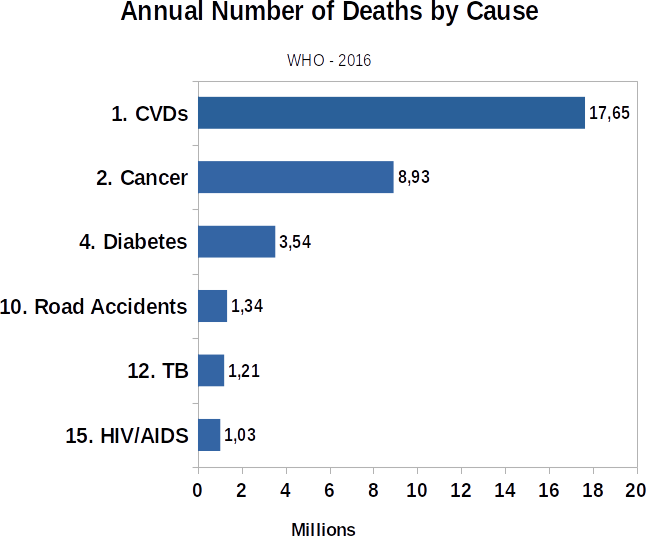
\includegraphics[width=\textwidth,height=0.6\textheight]{AAUgraphics/who.png}
  	 	\end{figure}
  	 }
  	
  	 
  	 % Image on second step
  	 
     \only<2>{ 
     	
     	\begin{figure}
  	 		\centering
  			
\includegraphics[scale=0.20]{AAUgraphics/ausc3.png}
  			
  		\end{figure}
      }
     
      % Image on 3rd step
  
      \only<3>{ 
    	
    	\begin{figure}
    		\centering
    		
\includegraphics[scale=1]{AAUgraphics/confused.jpg}
    	\end{figure}
           
           \vspace{-0.8cm}
           
        \begin{figure}
        	
        	\centering
        	
\includegraphics[width=\textwidth]{AAUgraphics/confstats.png}
        	\caption{\scalebox{.6}{Correct diagnosis using CA  in USA, Canada \& UK respectively.}}
        
        \end{figure}
    	}
    
       % Image on 4th Step
       
       \only<4>{ 
       	
       	\begin{figure}[t]
       		
       		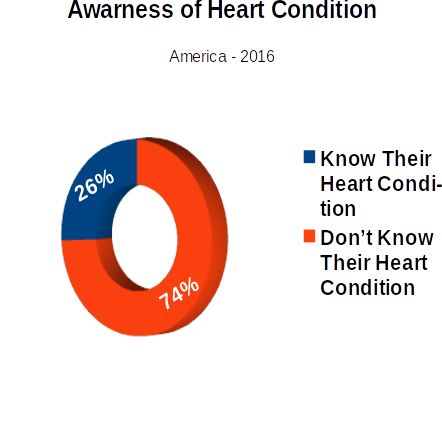
\includegraphics[width=\textwidth,height=0.7\textheight]{AAUgraphics/aware2.png}
       		
       	\end{figure}
       }
   
   
  \end{columns}

  \only<5>{
  	\vspace{-0.8\textheight}
      % \scalebox{1.5}
     {\Large Easily accessible \& reliable heart diagnosis systems would help reduce deaths due to CVDs.}

     }
  
\end{block}
\end{frame}
%%%%%%%%%%%%%%%%

	%\subsection{License}
	%% the license
	%\begin{frame}{Introduction}{License}
	%  \begin{itemize}
	%
	%  \end{itemize}
	%\end{frame}
	
%%%%%%%%%%%%%%%%

\section{Objectives}
% Kgwekgwe ya taba.
\begin{frame}{Objectives}

	\begin{itemize}
	
		\item<1-> To segment Heartbeat sounds (HSs) based on the location \\of S1 (lub) S2 (dub) in Normal HSs.
	

	\end{itemize}
	{	\begin{figure}
			\centering
			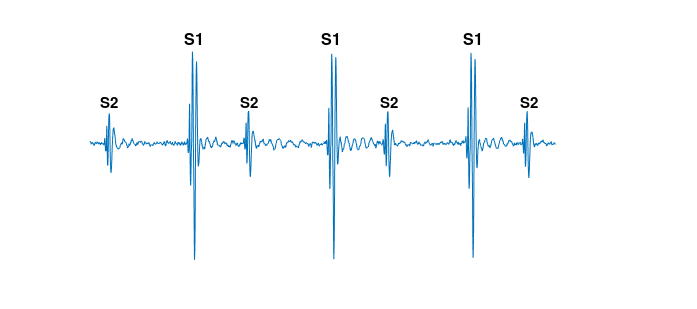
\includegraphics[width=0.75\textwidth,height=0.25\textheight]{AAUgraphics/s1s2s1wc.png}
		\end{figure}
	}

   \pause
   
   \begin{itemize}
   	
   		\item<2-> Create models that will enable preliminary screening of CVDs	
   	
   \end{itemize}
   
   	{	\begin{figure}
   			\centering
   			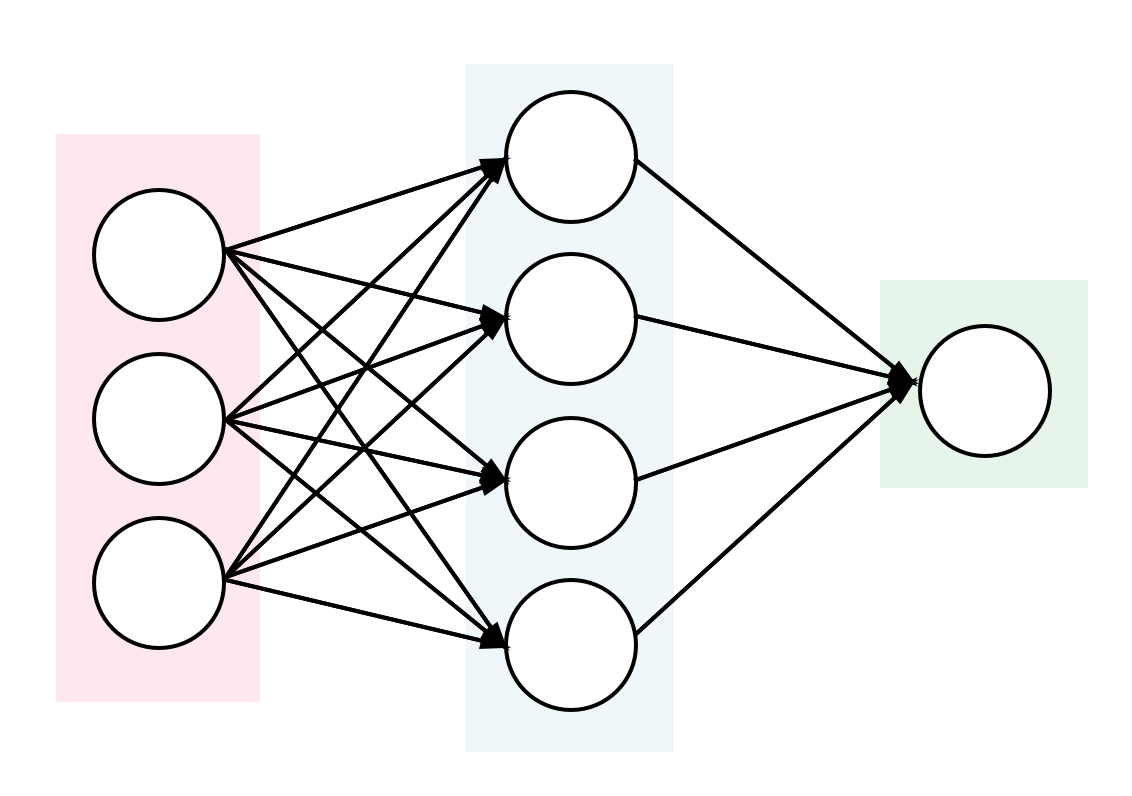
\includegraphics[width=0.5\textwidth,height=0.35\textheight]{AAUgraphics/classification2.png}
   		\end{figure}
   	}


\end{frame}

%%%%%%%%%%%%%%%%

\section{User Interface}
\subsection{Loading the Theme and Theme Options}
% list of the themes and options
\begin{frame}{User Interface}{Loading the Theme and Theme Options}
  \begin{block}{The Presentation Theme}
    It is very simple to load the presentation theme. Just type\\
    {\tt \textbackslash usetheme[<options>]\{AAUsimple\}}\\
    which is exactly the same way other beamer presentation themes are loaded. The presentation theme loads the inner, outer and color AAU Simple theme files and passes the {\tt <options>} on to these files.
  \end{block}
  \begin{block}{The Inner Theme}
    You can load the inner theme directly by\\
    {\tt \textbackslash useinnertheme\{AAUsimple\}}\\
    and it has no options.
  \end{block}
\end{frame}
%%%%%%%%%%%%%%%%

% list of the themes and options
\begin{frame}{User Interface}{Loading the Theme and Theme Options}
  \begin{block}{The Outer Theme}
    You can load the outer theme directly by\\
    {\tt \textbackslash useoutertheme[<options>]\{AAUsimple\}}\\
    Currently, the theme options are
  \begin{itemize}
    \item {\tt progressstyle=\{fixedCircCnt, movCircCnt, or corner\}}: set how the progress is illustrated. The value {\tt fixedCircCnt} is the default. 
    \item {\tt rotationcw}: set the direction of the rotation of the progress circle to clockwise instead of counterclockwise. This option has only effect for the circular progress bars.
    \item {\tt shownavsym}: show the navigation symbols
  \end{itemize}
  \end{block}
\end{frame}
%%%%%%%%%%%%%%%%

% list of the themes and options
\begin{frame}{User Interface}{Loading the Theme and Theme Options}
  \begin{block}{The Color Theme}
    You can load the color theme directly by\\
    {\tt \textbackslash usecolortheme\{AAUsimple\}}\\
    and it has no options.
  \end{block}
  \pause
  \begin{block}{The Color Element {\tt AAUsimple}}
    The color theme defines a new beamer color element named {\tt AAUsimple} whose foreground and background colors are
    \begin{itemize}
      \item fg: {\usebeamercolor[fg]{AAUsimple}light blue (\{RGB\}\{194,193,204\})}
      \item bg: {\usebeamercolor[bg]{AAUsimple}dark blue (\{RGB\}\{33,26,82\})}
    \end{itemize}
    You can use these colors in the standard beamer way by using the command
    {\tt \textbackslash usebeamercolor[<fg or bg>]\{AAUsimple\}}. See the beamer manual for instructions.\\
 \pause Note that this version of the theme is an official AAU version and is in accordance with the \chref{http://aau.designguides.dk/}{AAU design guide}. However, you can easily change it (including the colour of the logo) by following the steps in {\tt beamercolorthemeAAUsimple.sty}.
  \end{block}
\end{frame}
%%%%%%%%%%%%%%%%

\subsection{Modifying the theme}
% how to modify the theme
{\setbeamercolor{AAUsimple}{fg=gray!50,bg=orange!50}
 \setbeamercolor{structure}{fg=red}
 \setbeamercolor{frametitle}{use=structure,fg=structure.fg}
 \setbeamercolor{normal text}{bg=gray!20}
\begin{frame}{User Interface}{Modifying the Theme}
  \begin{itemize}
    \item<1-> The default configuration of fonts, colors, and layout complies with the \chref{http://aau.designguides.dk}{AAU design guidelines} and is the \alert{official} version of the theme.
    \item<2-> However, you can modify specific elements of the theme through the templates provided by the beamer class. Please refer to the beamer user manual for instructions.
    \item<3-> For example, on this slide the following commands have been used
      \begin{itemize}
        \item Change the header colours:\\
        {\tt \textbackslash setbeamercolor\{AAUsimple\}\{fg=blue!20,bg=red!50\}}
        \item Change the color of the structural elements:\\
        {\tt \textbackslash setbeamercolor\{structure\}\{fg=black\}}\\
        \item Change the frame title text color:
        {\tt \textbackslash setbeamercolor\{frametitle\}\{use=structure, fg=structure.fg\}}
        \item Change the background color of the text
        {\tt \textbackslash setbeamercolor\{normal text\}\{bg=gray!20\}}
      \end{itemize}
  \end{itemize}
\end{frame}}
%%%%%%%%%%%%%%%%

\subsection{AAU Waves}
% the AAU Waves background
\begin{frame}{User Interface}{The AAU Waves Background Image}
\begin{block}{The AAU Waves Background Image}
\begin{itemize}
  \item<1-> In this documentation, the title page frame and the last frame have the AAU waves as the background image. The AAU waves background image can be added to any single frame by wrapping a frame in the following way\\
  {\tt \{\textbackslash aauwavesbg\\
    \textbackslash begin\{frame\}[<options>]\{Frame Title\}\{Frame Subtitle\}\\
    \ldots\\
    \textbackslash end\{frame\}\}}
  \item<2-> Ideally, I would like to create a new frame option called {\tt aauwavesbg} which can enable the AAU waves background. However, I have not been able to figure out how such an option can be added. If you know how this can be done, please contact me.
\end{itemize}
\end{block}
\end{frame}
%%%%%%%%%%%%%%%%

\subsection{Widescreen Support}
% Widescreen Support
\begin{frame}{User Interface}{Widescreen Support}
\begin{block}{Widescreen Support}
  Newer projectors and almost any modern TV support a widescreen format such as 16:10 or 16:9. Beamer (>= v. 3.10) supports various aspect ratios of the slides. According to section 8.3 on page 77 of the Beamer user guide v. 3.10, you can write\\
{\tt\textbackslash documentclass[aspectratio=1610]\{beamer\}}\\
to get slides with an aspect ratio of 16:10. You can also use 169, 149, 54, 43 (default), and 32 to get other aspect ratios.
\end{block}
\end{frame}
%%%%%%%%%%%%%%%%


\section{Feedback}
\subsection{Known Problems}
% known problems
\begin{frame}{Feedback}{Known Problems}
  \begin{description}
    \item[More than 50 slides] Internally, TeX cannot work with numbers exceeding +/-16
  \end{description}
\end{frame}
%%%%%%%%%%%%%%%%

\subsection{Bugs, Comments and Suggestions}
% help me iron out the bugs or give me some comment and suggestions
\begin{frame}{Feedback}{Bugs, Comments and Suggestions}
  \begin{itemize}
    \item<1-> There are probably still some bugs in the theme. If you should find one, then please let me know. No bug is too small!
    \item<2-> Also, please contact me, if you have some exciting new ideas or just some simple usability improvements.
  \end{itemize}
\end{frame}
%%%%%%%%%%%%%%%%

\subsection{Contact Information}
% contact information
\begin{frame}{Feedback}{Contact Information}
In case you have any comments, suggestions or have found a bug, please do not hesitate to contact me. You can find my contact details below.
  \begin{center}
    \insertauthor\\
    \chref{http://kom.aau.dk/~jkn}{http://kom.aau.dk/\textasciitilde jkn}\\
    Niels Jernes Vej 12, A6-309\\
    9220 Aalborg Ø
  \end{center}
\end{frame}
%%%%%%%%%%%%%%%%

{\aauwavesbg
\begin{frame}[plain,noframenumbering]
  \finalpage{Thank you for using this theme!}
\end{frame}}
%%%%%%%%%%%%%%%%

\end{document}
